
\subsection{Professional Quality Plots}
\begin{frame}
\frametitle{Professional Quality Plots}
\begin{columns}
\begin{column}{4cm}
\begin{itemize}
	\item Annotations
	\item Colors
	\item Lighting
	\item Views
\end{itemize}
\end{column}
\begin{column}{6cm}
	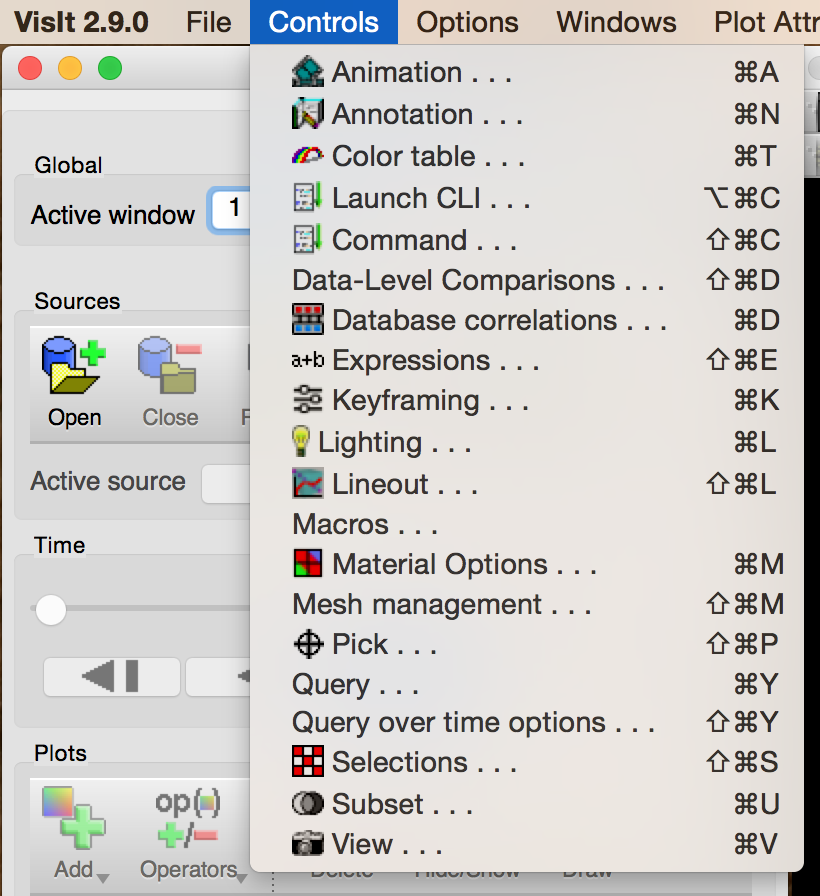
\includegraphics[width=\columnwidth]{figs/visit-guis/visit_ctrls}
\end{column}
\end{columns}
\end{frame}

\subsubsection{Annotations}
\begin{frame}
\frametitle{Annotations}
\begin{columns}
\begin{column}{5cm}
\begin{block}{Annotations}
\begin{itemize}
	\item objects in the viz-window
		that convey infromation about the plots
	\item make clear what is being visualized and make
		the visualization appear more polished
\end{itemize}
\end{block}
\end{column}
\begin{column}{5cm}
\begin{block}{Types of Annotations}
\begin{itemize}
        \item Database name
        \item User name
	\item plot legends
	\item plot axes and labels (2d \& 3d)
	\item 3d triad
	\item 2d, 3d text
	\item time slider
	\item images
	\item line and arrows
\end{itemize}
\end{block}
\end{column}
\end{columns}
\end{frame}


\begin{frame}
\frametitle{Annotation Window}
\begin{columns}
\begin{column}{5cm}
\begin{itemize}
        \item General annotations
        \item 2D axes settings
        \item 3D axes settings
        \item Array axis settings
	\item Color and Backgrounds
	\item Objects (legend, timr slider, ...)
\end{itemize}
\end{column}
\begin{column}{5cm}
        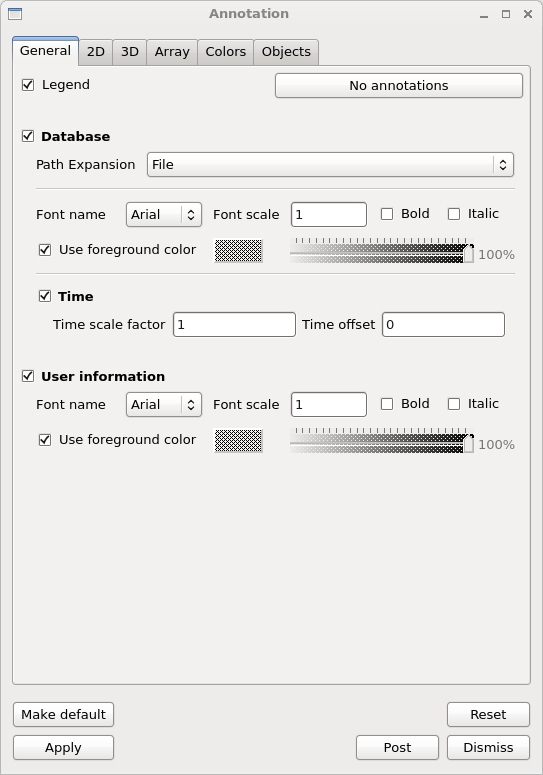
\includegraphics[width=\columnwidth]{figs/visit-guis/visit_annot}
\end{column}
\end{columns}
\end{frame}


\begin{frame}
\frametitle{2D \& 3D Annotations}
\begin{columns}
\begin{column}{5.75cm}
	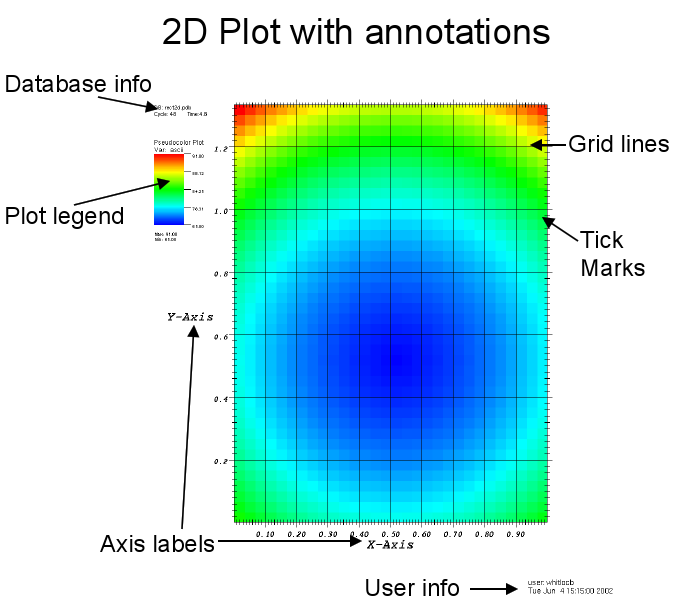
\includegraphics[width=\columnwidth]{figs/visit-guis/visit_2d-objects}

	\vspace{2mm}
	\textcolor{DarkBlue}{\ding{224}}
        \framebox{Controls} $\rightarrow$ \framebox{\bf Annotation...}
		\ding{232}[\textcolor{DarkBlue}{\bf "2D" tab}]
\end{column}
\begin{column}{5.25cm}
        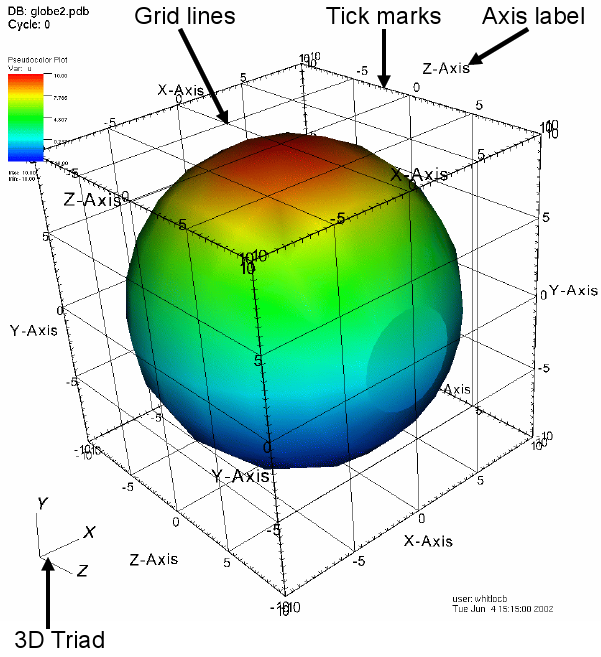
\includegraphics[width=\columnwidth]{figs/visit-guis/visit_3d-objects}

	\vspace{2mm}
        \textcolor{DarkBlue}{\ding{224}}
        \framebox{Controls} $\rightarrow$ \framebox{\bf Annotation...}
		\ding{232}[\textcolor{DarkBlue}{\bf "3D" tab}]
\end{column}
\end{columns}
\end{frame}


\begin{frame}
\frametitle{Colors and Backgrounds}
\begin{columns}
\begin{column}{6cm}
        \textcolor{DarkBlue}{\ding{224}}
        \framebox{Controls} $\rightarrow$ \framebox{\bf Annotation...}

	\hspace{5mm}
	\ding{232}[\textcolor{DarkBlue}{\bf "Colors" tab}]

	\begin{itemize}
		\item set background/foreground
		\item Backgroun styles:
		\begin{itemize}
		\item solid
		\item gradient
		\item image (flat image)
		\item image sphere (warped image, that rotates witht the view)
		\item number of repetitions
		\end{itemize}
	\end{itemize}

	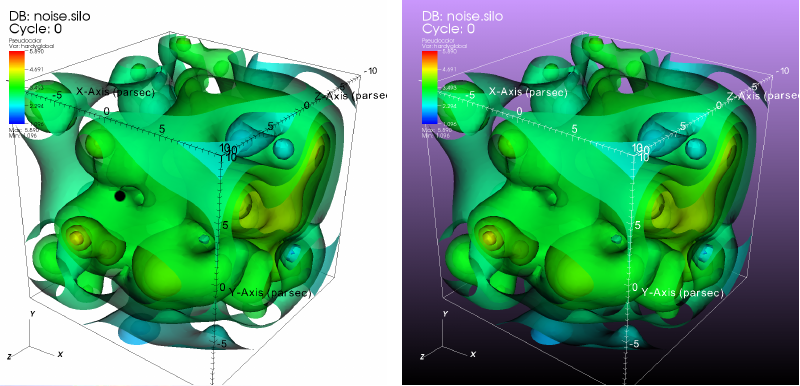
\includegraphics[width=\columnwidth]{figs/visit-pract/VisIt_backgrounds}
\end{column}
\begin{column}{4.75cm}
        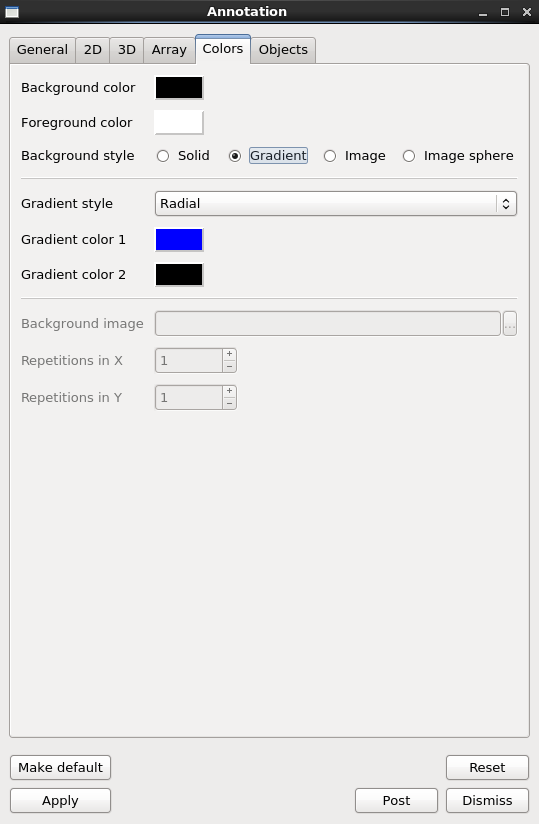
\includegraphics[width=\columnwidth]{figs/visit-guis/visit_annot-colors}
\end{column}
\end{columns}
\end{frame}


\begin{frame}
\frametitle{Annotation Objects}
\begin{columns}
\begin{column}{5.5cm}
        \textcolor{DarkBlue}{\ding{224}}
        \framebox{Controls} $\rightarrow$ \framebox{\bf Annotation...}

        \hspace{5mm}
        \ding{232}[\textcolor{DarkBlue}{\bf "Objects" tab}]

        \begin{itemize}
                \item 2D/3D Text
		\item 2D/3D Lines
                \item Time Slider
                %\begin{itemize}
                %\item shows progress through an animation
                %\end{itemize}
		\item Image
        \end{itemize}

	\centering
	\vspace{-2mm}
	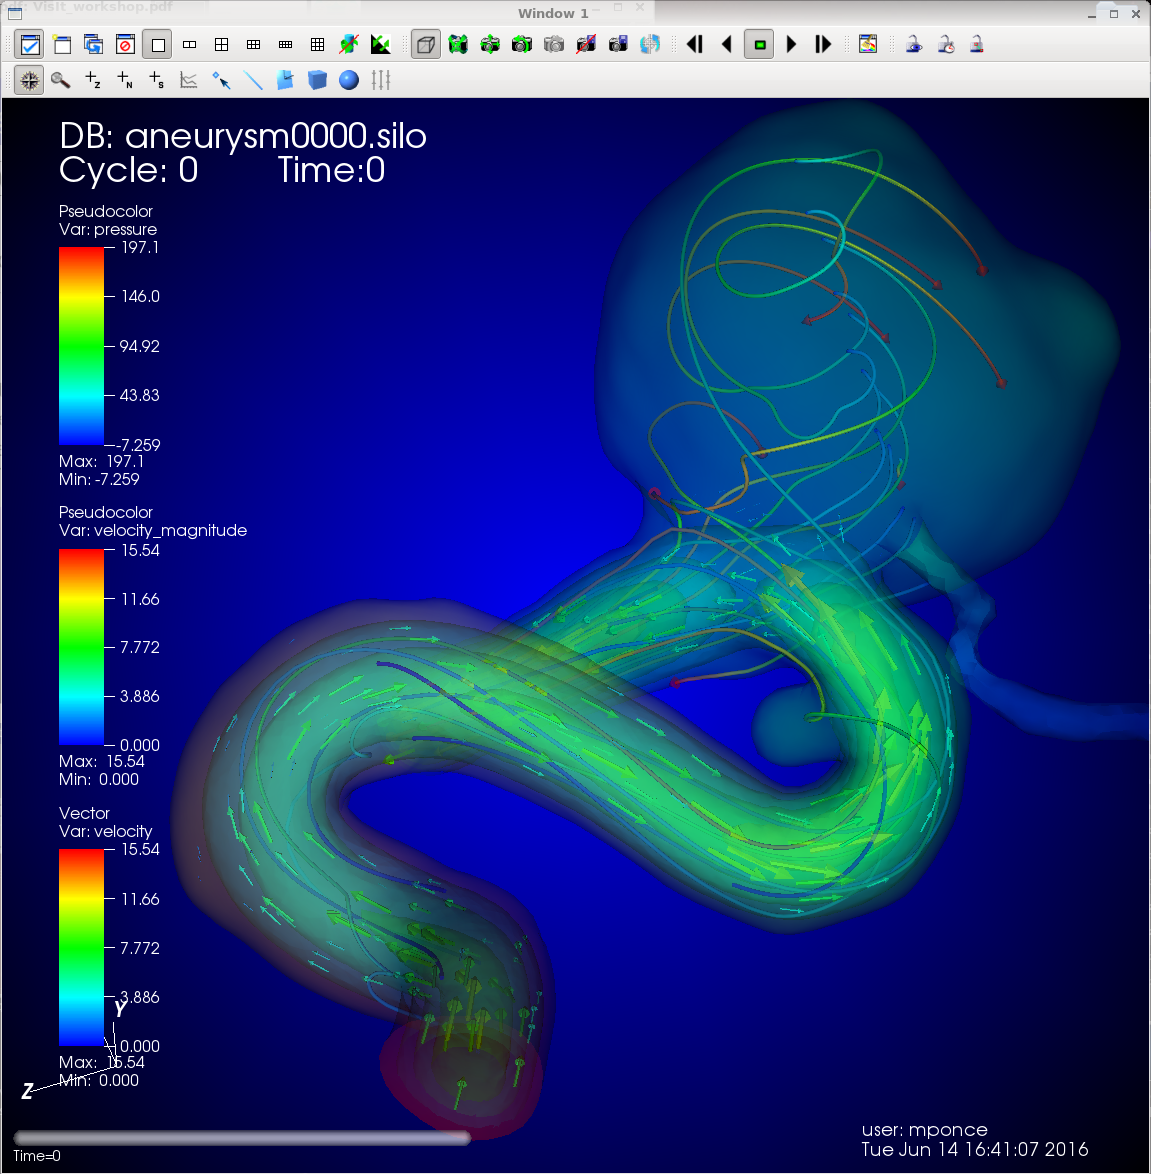
\includegraphics[width=.855\columnwidth]{figs/visit-pract/VisIt_timeSlider}
\end{column}
\begin{column}{4.5cm}
        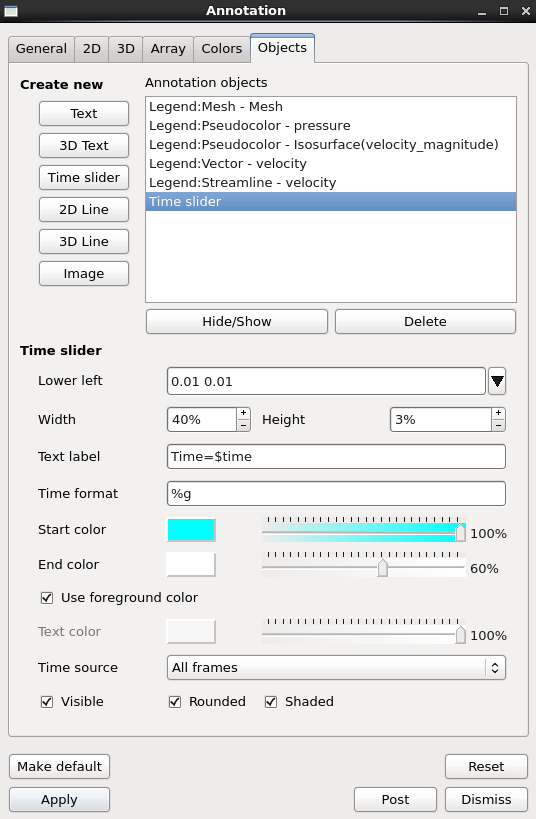
\includegraphics[width=\columnwidth]{figs/visit-guis/visit_annot-objects}
\end{column}
\end{columns}
\end{frame}


\subsubsection{Lighting}
\begin{frame}
\frametitle{Lighting}
\vspace{-5mm}
\begin{columns}[T]
\begin{column}{6cm}
\begin{itemize}
        \item Lighting affects the brightness of plots
        \item 3D visualizations may require multiple \textit{light sources}
        \item VisIt allows up to 8 light sources
        \item Each light source can be positioned and colored
\end{itemize}

	\pause
        \textcolor{DarkBlue}{\ding{224}}
        \framebox{Controls} $\rightarrow$ \framebox{\bf Lighting...}

	\pause
        \vspace{-1.5mm}
	\begin{block}{}
	\begin{itemize}
	\item ~[Edit]: configure light sources
	\item ~[Preview]: all sources are visible
	\end{itemize}

	\centering
	\vspace{-2mm}
	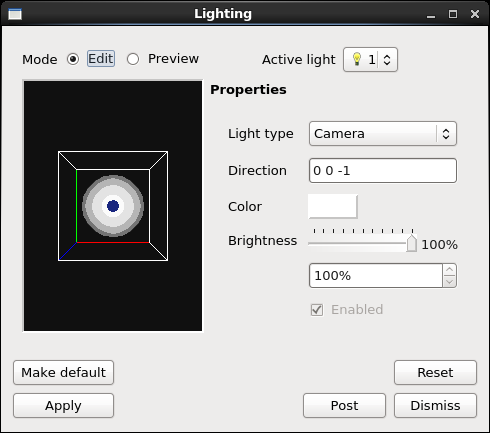
\includegraphics[width=.65\columnwidth]{figs/visit-guis/visit_lighting}
	\end{block}
\end{column}
\begin{column}{5.5cm}
	\pause
        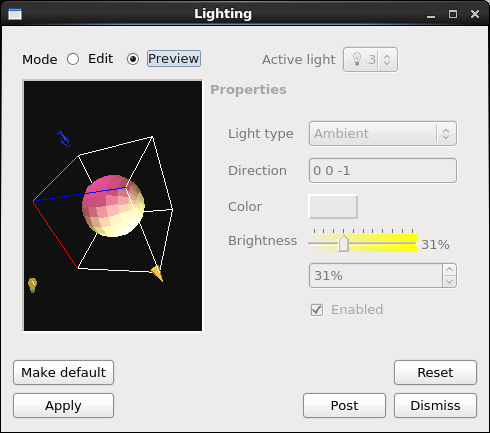
\includegraphics[width=.85\columnwidth]{figs/visit-guis/visit_lighting2}

	\vspace{-2mm}
	\begin{block}{}
	\begin{itemize}
		\item only the active light can be modified
		\item once a light has been selected, you can change its props.
		\item Types of lights: Ambient, Camera, Object Light
		\item Position, Color, Brightness
	\end{itemize}
	\end{block}
\end{column}
\end{columns}
\end{frame}


\subsubsection{Views}
\begin{frame}
\frametitle{View}
\vspace{-2.5mm}
\begin{columns}
\begin{column}{12.5cm}
\begin{itemize}
        \item the ``view'' can be set \textit{interactively} in the viz-window (click and drag, ...)
        \item or using a ``View Window'', to specify exactly the configuration view
\end{itemize}
\end{column}
\end{columns}

        \pause
        \textcolor{DarkBlue}{\ding{224}}
        \framebox{Controls} $\rightarrow$ \framebox{\bf View...}

\vspace{-1mm}
\begin{columns}[T]
\begin{column}{3cm}
        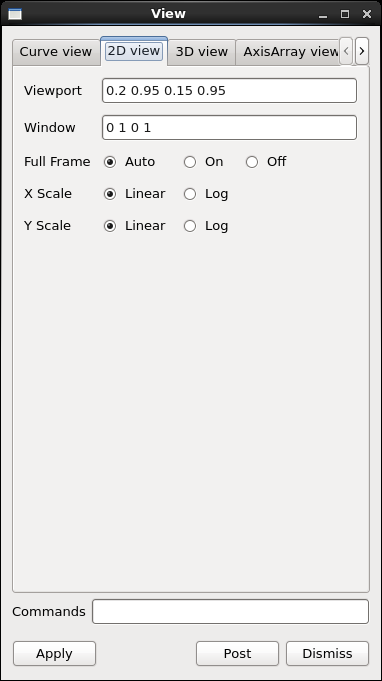
\includegraphics[width=.9\columnwidth]{figs/visit-guis/visit_view2d}
\end{column}
\begin{column}{3cm}
	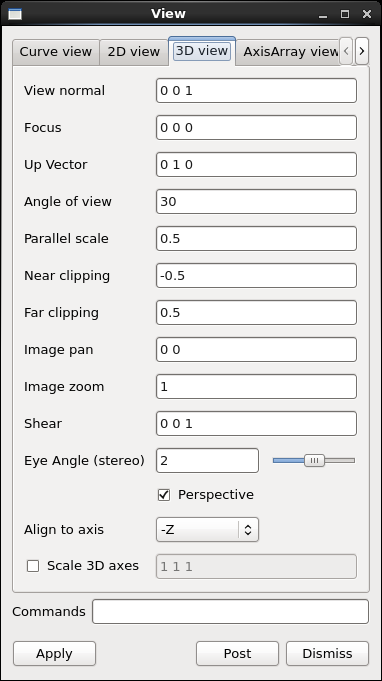
\includegraphics[width=.9\columnwidth]{figs/visit-guis/visit_view3d}
\end{column}
\begin{column}{3cm}
	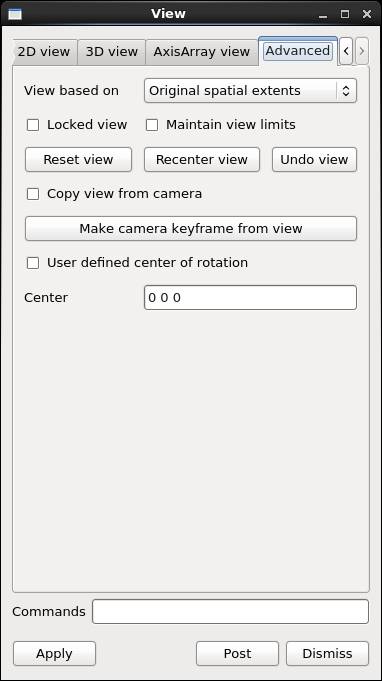
\includegraphics[width=.9\columnwidth]{figs/visit-guis/visit_viewAdv}
\end{column}
\end{columns}

\begin{itemize}
	\item ``\textbf{Locked view}'': when the view changes in any locked window, all other locked window readjust to it
	\item accessible from the [Advanced] tab or ``Lock View'' tool on the viz-window
\end{itemize}

\end{frame}



\subsection{Movies Generation}

\begin{frame}
\frametitle{Movie Generation}

\end{frame}
